\documentclass[runningheads]{llncs}
\usepackage[T1]{fontenc}
\usepackage{graphicx}
\usepackage{subfigure}
\usepackage{subcaption}


\begin{document}
%
\title{Algoritmo genetico binario y real para el problema de la esfera y la función de  Rastrigin.}
\author{Angel García Báez \inst{1}}
%
\institute{Universidad Veracruzana. Instituto de Investigaciones en Inteligencia Artificial}
\maketitle              % typeset the header of the contribution
%
%
%
\section{Detalles de las implementaciones}

Se busca minimizar mediante algoritmos genéticos la función de la esfera y la de Rastrigin en 10 Dimensiones. Para cada uno de los problemas, se implemento un algoritmo genético real y otro binario con las características mencionadas en la figura 1.C. 

Se decidió usar un mismo conjunto de parametros en comun para ambos problemas y para ambas representaciones, con el fin de mantener las comparativas equilibradas. Nota: Se implemento elitismo en ambas representaciones.

\begin{figure}[htbp]
	\centering
	\subfigure[Problema 1: Esfera en 3D]{
		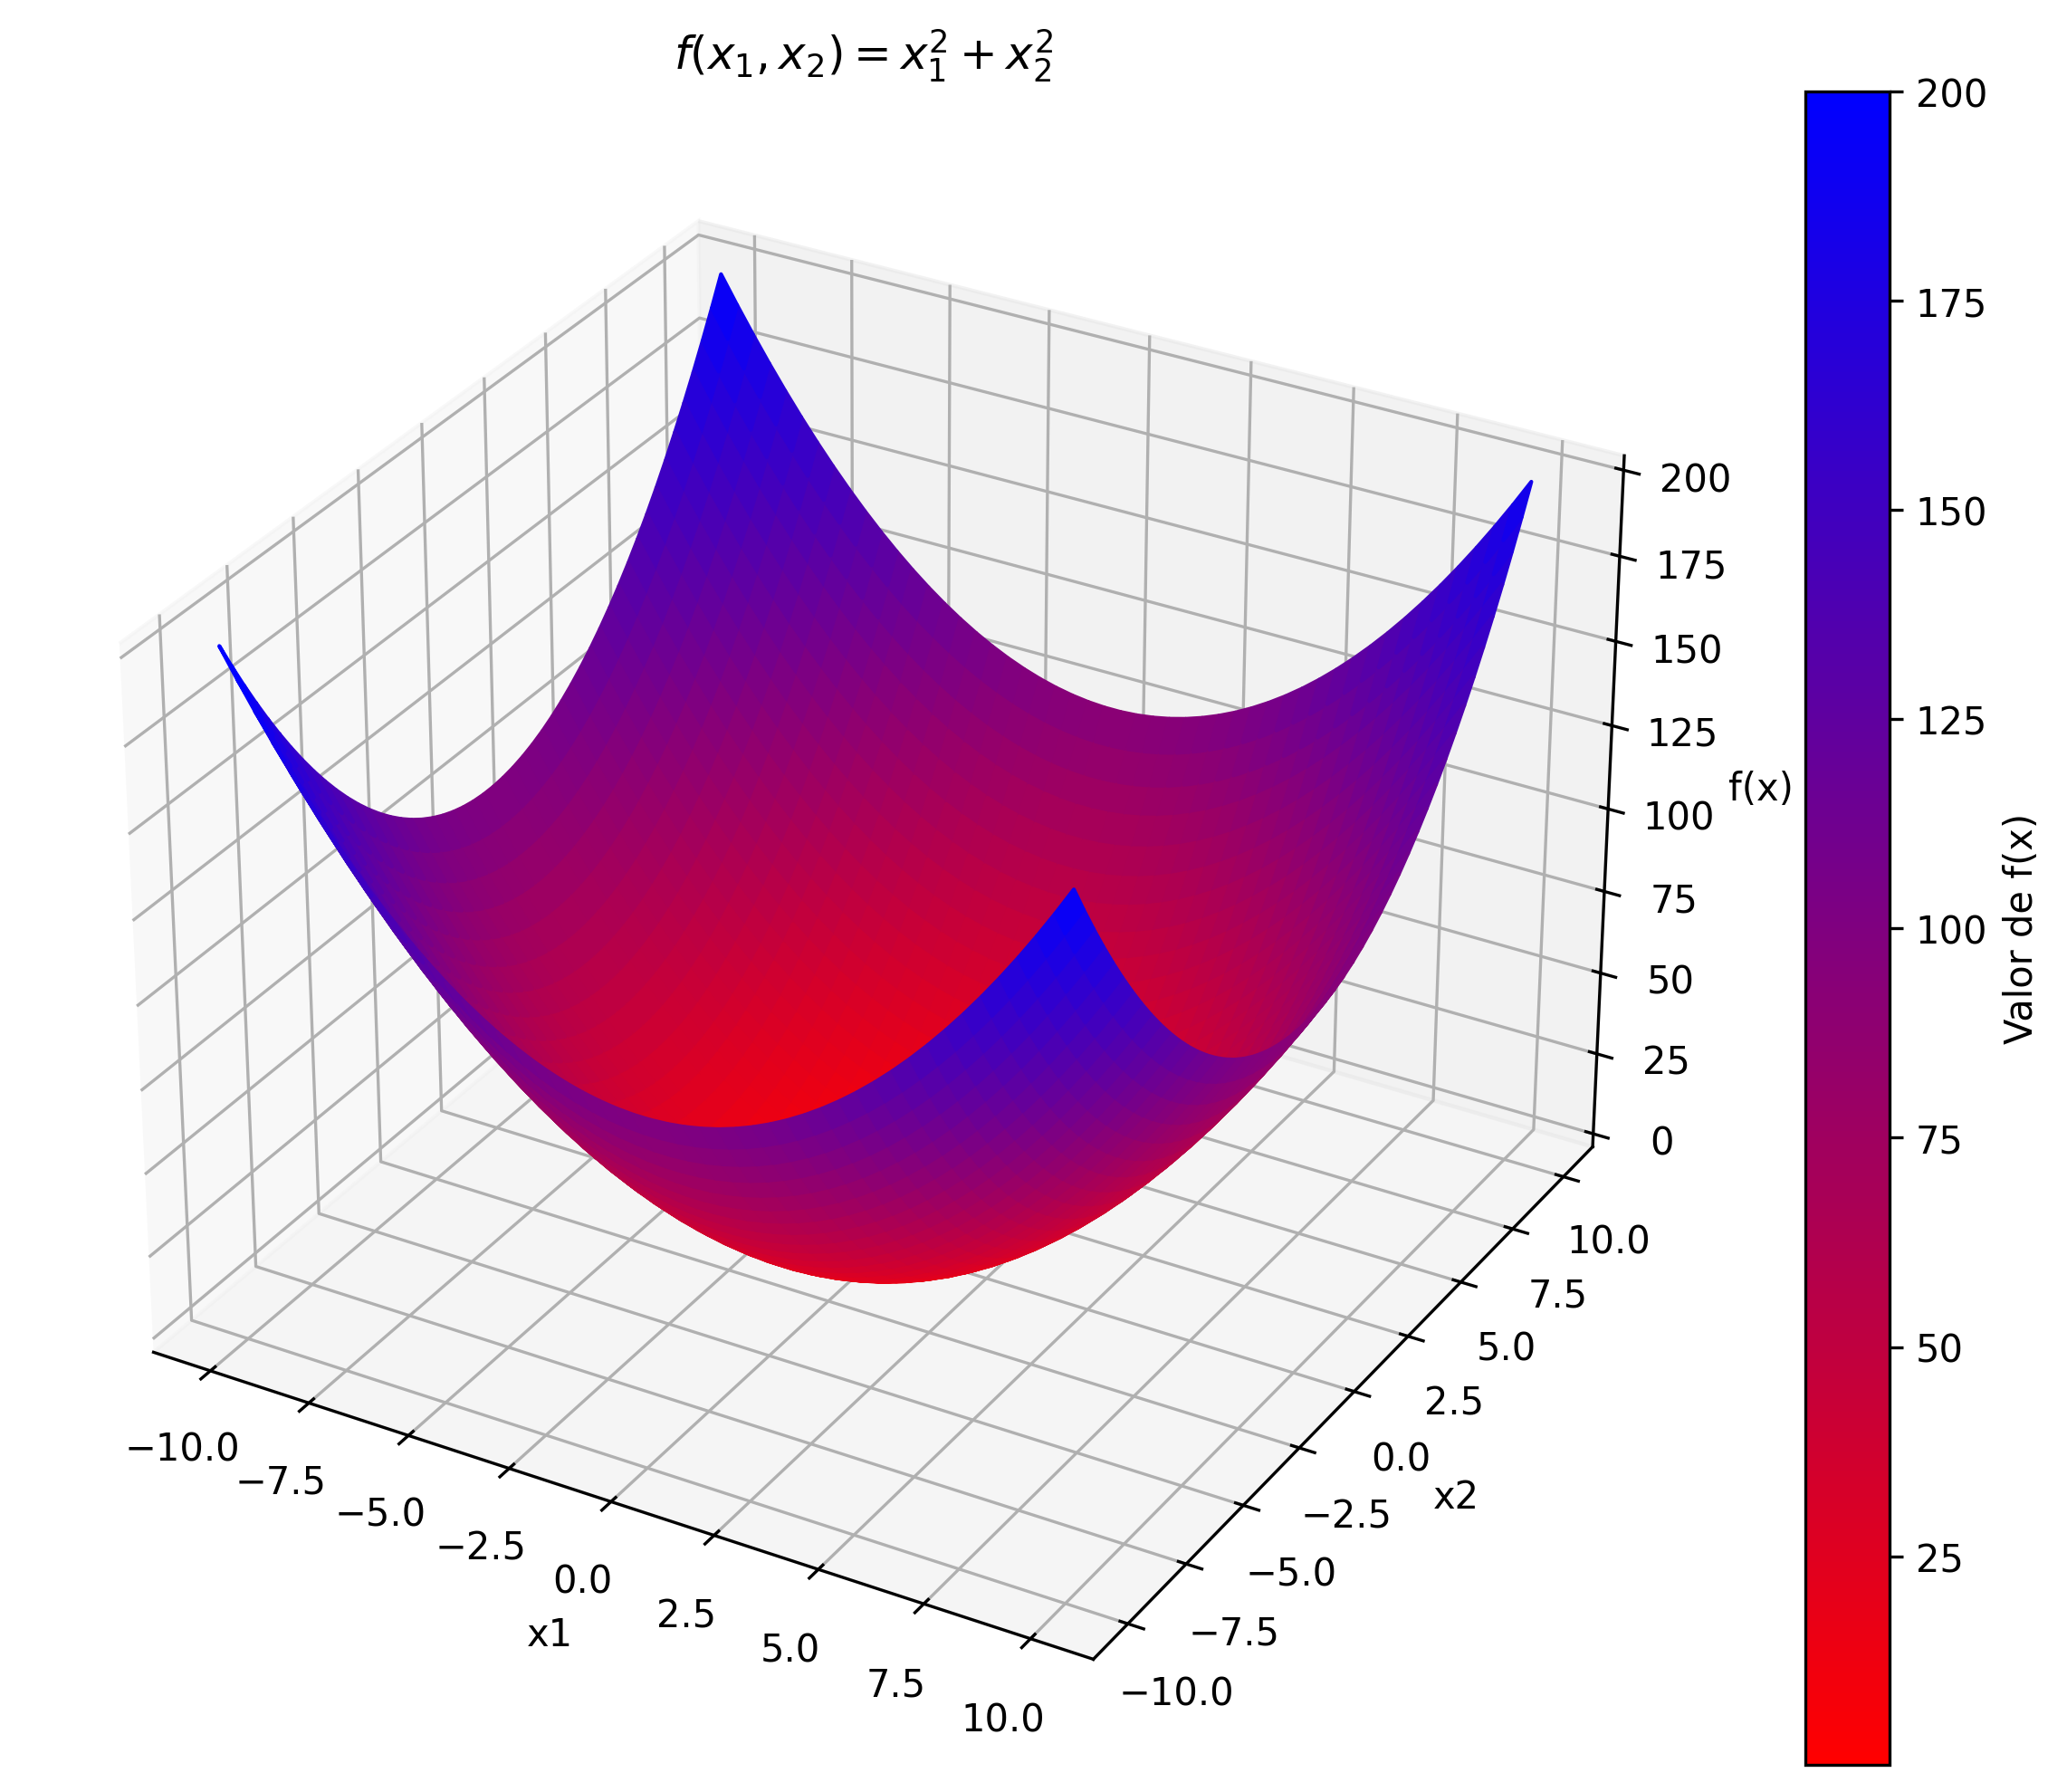
\includegraphics[width=0.23\textwidth]{IMG/P1.png}
		\label{fig:G1}
	}
	\hspace{0.01\textwidth} % espacio muy pequeño entre figuras
	\subfigure[Problema 2: Función  Rastrigin en 3D]{
		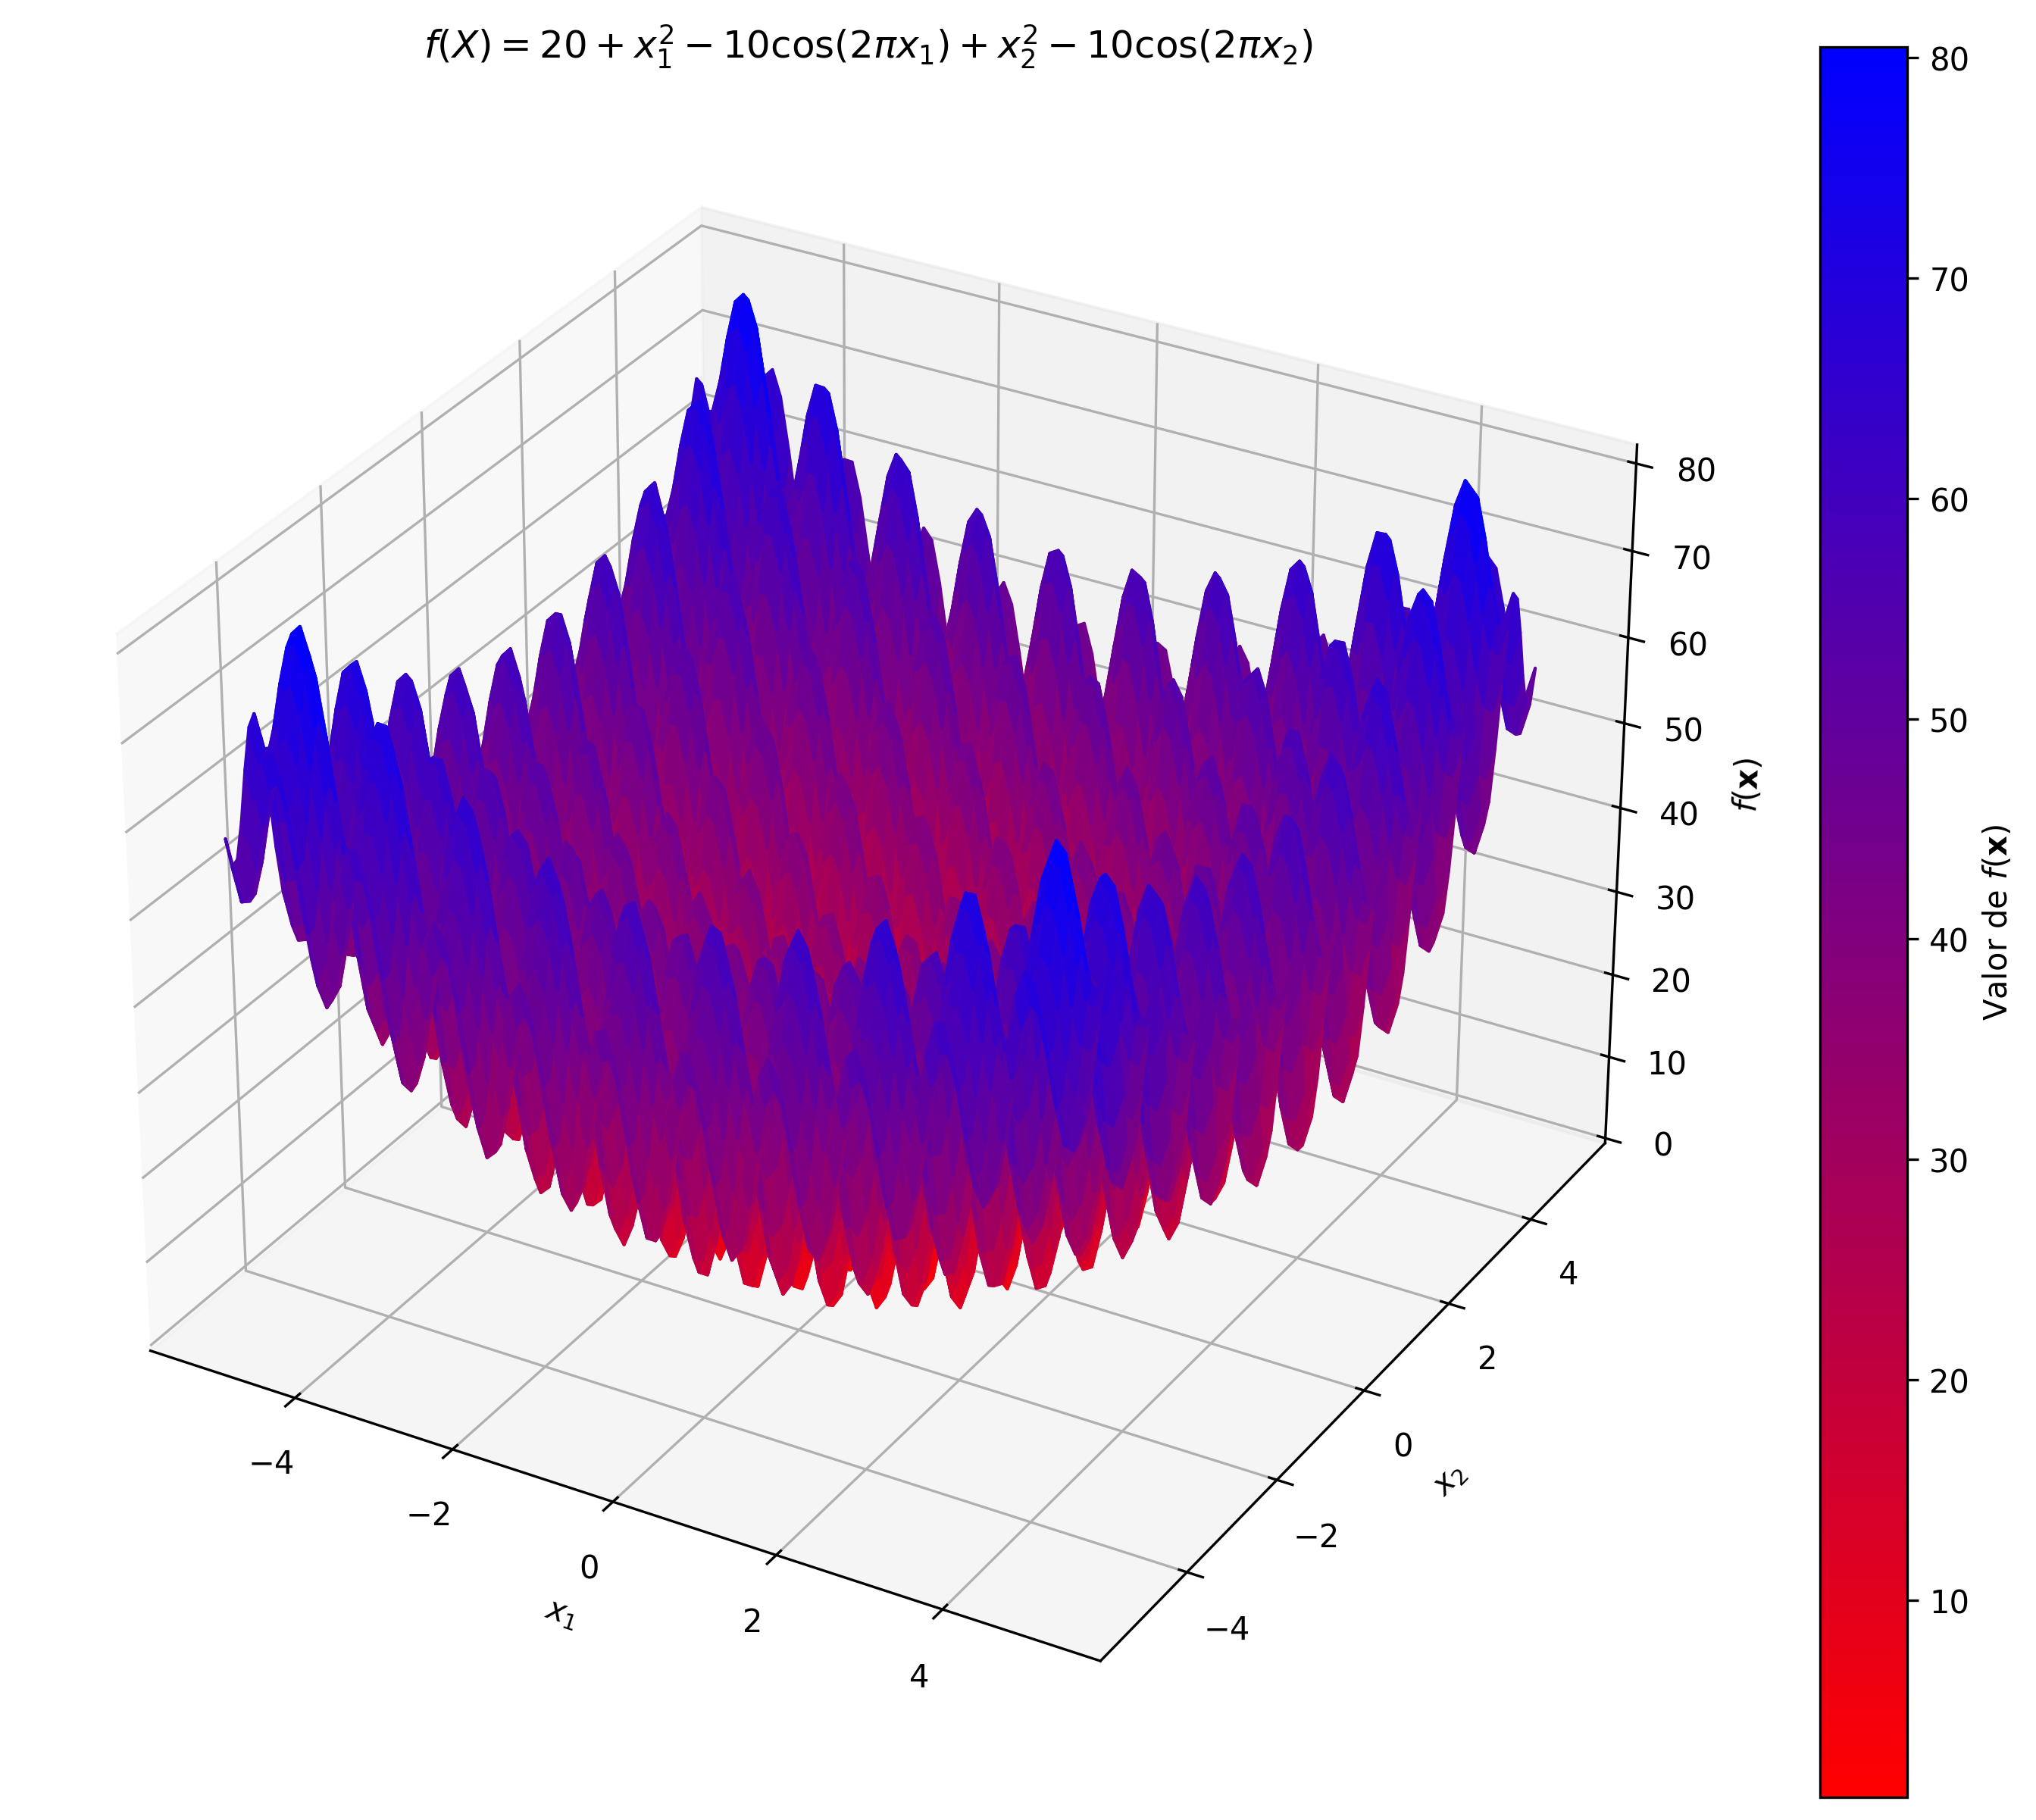
\includegraphics[width=0.23\textwidth]{IMG/P2.png}
		\label{fig:G2}
	}
		\hspace{0.01\textwidth} % espacio muy pequeño entre figuras
	\subfigure[Diseño de los algoritmos real y binarios]{
		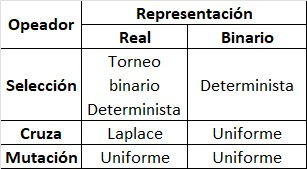
\includegraphics[width=0.30\textwidth]{IMG/R3.jpg}
		\label{fig:G3}
	}
	\vspace{-0.5em} % reducir espacio vertical antes del caption
	\caption{Funciones objetivo y diseño de los algoritmos geneticos}
	\label{fig:modelos}
\end{figure}

Se manejaron los siguientes parámetros para ambas representaciones, con la particularidad de que $b$ pertenece unicamente al operador laplaciano de la representación real.

Parámetros: pobsize = 30 | ngen = 2000 | PC = 0.8 | PM = 0.01 | b = 0.001

Se realizaron 30 corridas aleatorias con los mismos parámetros, se obtuvieron estadísticas descriptivas.

\begin{figure}[htbp]
	\centering
	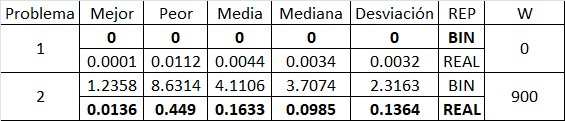
\includegraphics[width=0.60\textwidth]{IMG/R4.jpg}
	\caption{Resumen estadístico con W de wilcoxon}
	\label{fig:r4}
\end{figure}

\newpage

Posteriormente, se muestran los resultados de los mejores sujetos por cada una de las 30 corridas aleatorias de cada algoritmo y problema.


\begin{figure}[htbp]
	\centering
	\subfigure[Representación Real. Problema 1. ]{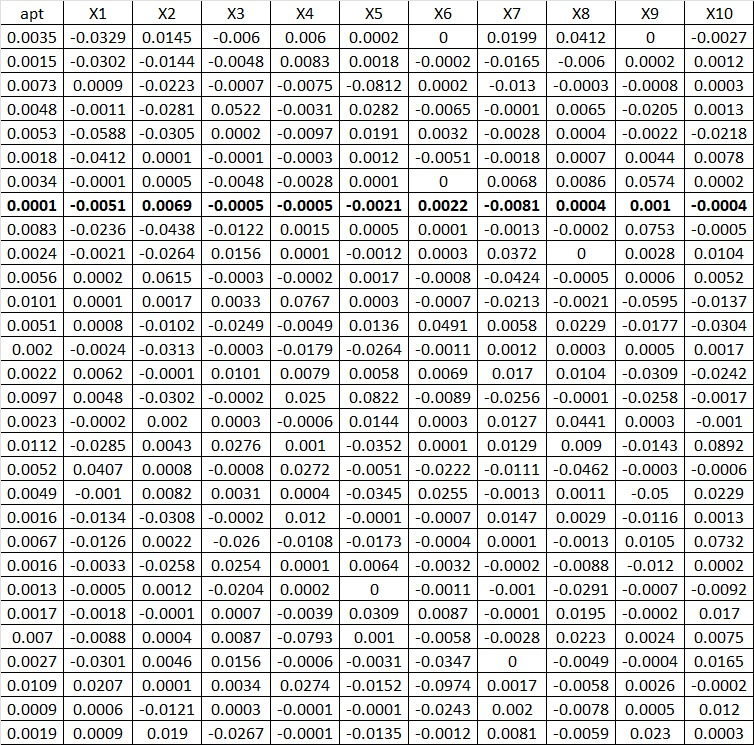
\includegraphics[width=0.35\textwidth]{IMG/RG1.jpg}}
	\subfigure[Representación Real. Problema 2.]{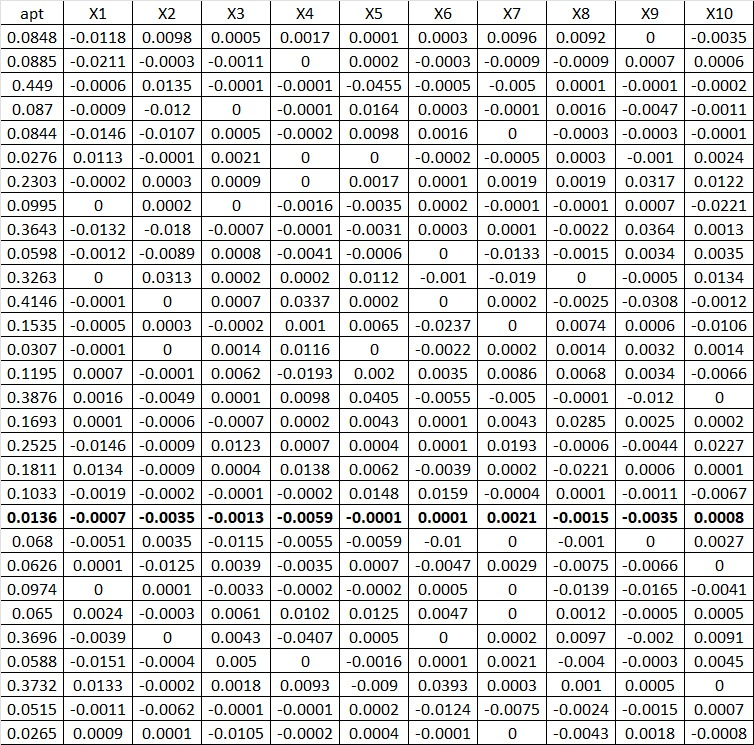
\includegraphics[width=0.35\textwidth]{IMG/RG2.jpg}}\\
	\subfigure[Representación Binaria Problema 1.]{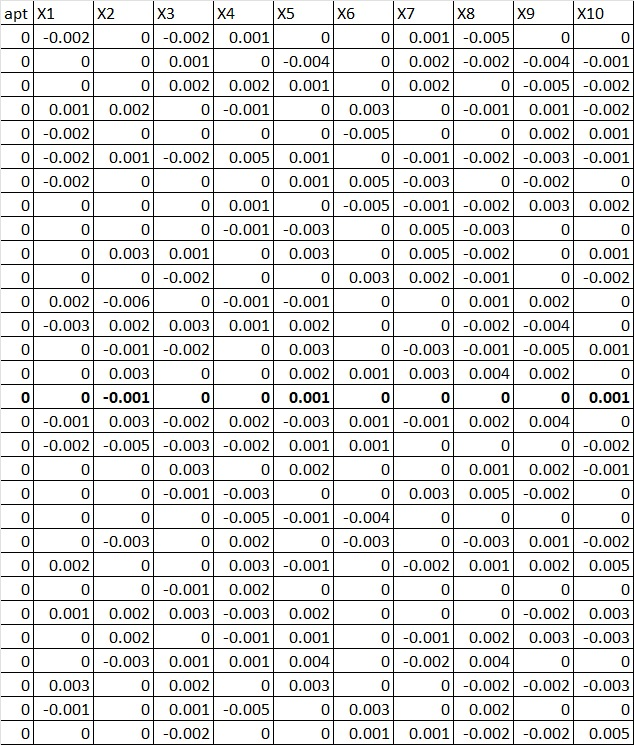
\includegraphics[width=0.35\textwidth]{IMG/RG3.jpg}}
	\subfigure[Representación Binaria Problema 2]{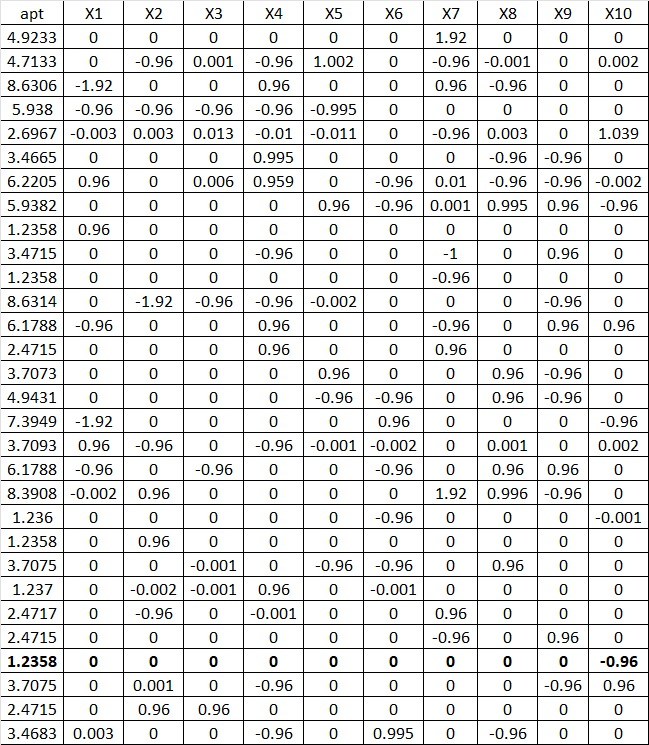
\includegraphics[width=0.35\textwidth]{IMG/RG4.jpg}}
	\caption{Mejores sujetos en 30 ejecuciones independientes.}
	\label{fig:rg_grid}
\end{figure}


\newpage

\begin{figure}[htbp]
	\centering
	\subfigure[Problema 1: Esfera]{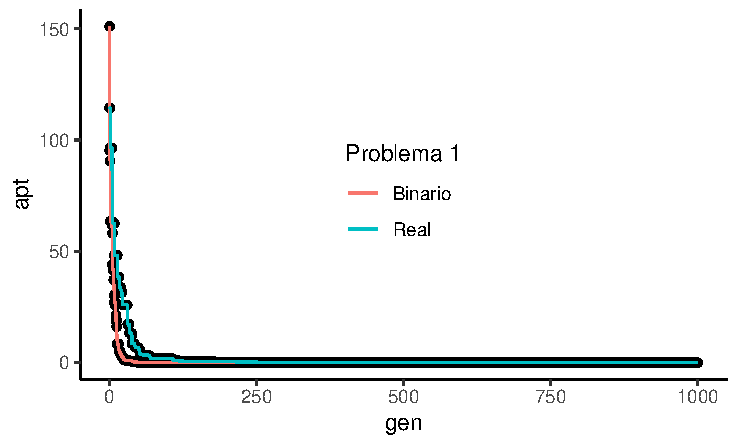
\includegraphics[width=0.45\textwidth]{IMG/CP1.pdf}}
	\hfill
	\subfigure[Problema 2: Esfera]{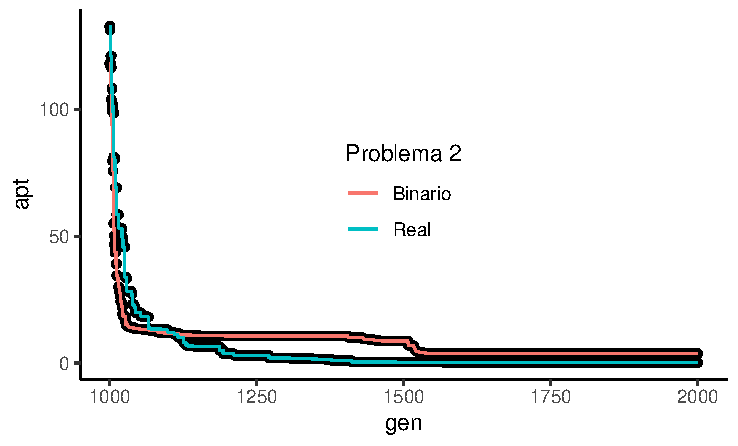
\includegraphics[width=0.45\textwidth]{IMG/CP2.pdf}}
	\caption{Comparativa entre algoritmos para la convergencia de la evaluación mediana.}
	\label{fig:convergencia}
\end{figure}



\section{Discusión de resultados}

Se encontraron diferencias significativas entre los resultados de las corridas aleatorias por problema para las representaciones real y binaria. El problema 1 es resuelto de forma más concisa con representación binaria, mientras que en el problema 2, es la representación real la que logra mejores resultados.

La implementación de los algoritmos fue más sencilla en el caso real, mientras que para el caso binario fue necesario implementar un sistema de codificación y decodificación basado en conversiones a números uniformes, esto se traduce en trabajo extra para el programa. Sin embargo, la implementación de los operadores sobre la representación real fue más rápida de implementar, al hacer unicamente pequeños cambios sobre los bits.

La calibración de parámetros fue más complicada en el caso binario, debido a que iba convergiendo de forma muy lenta a mejores soluciones pero es muy susceptible a la influencia que pueda aplicar el porcentaje de mutación, que puede mandar una solución buena a una solución pésima haciendo el cambio en un solo bit.

De forma general, la representación binaria permite una implementación más directa y limpia de los operadores genéticos pero al costo de llevar ese computo extra para hacer la codificación y decodificación de las cadenas binarias y la exhaustiva calibración de sus parámetros hasta lograr una combinación estable. 

Por otro lado, la representación real consigue que se puedan representar a los individuos de forma rápida y directa, al costo de que sus operadores pueden ser más detallosos de implementar, pero justo ahí en el fino detalle es donde radica otra de sus bondades, al tener como extra el parametro $b$, asociado a la cruza de laplace, le permite modular de mejor manera que tanto explota o explora el espacio de busqueda. Esto ultimo se refleja en sus resultados para el problema 2, que es un problema no lineal lleno de minimos locales, la evidencia obtenida muestra que se desempeña significativamente mejor en dicho problema a comparación del binario.





\end{document}
